\section{Tensão}

Para deslocar o elétron em um condutor determinado sentido é necessário trabalho
que é realizado por uma força eletromotriz (FEM) externa representada pela
bateria na Figura~\ref{fig:fig1}. Essa FEM também é conhecida como
\textit{tensão} ou \textit{diferença de potencial}. A tensão \( v_{ab} \) entre
dois pontos \( a \) e \( b \) em um circuito é a energia necessária para
deslocar uma carga unitária de \( a \) para \( b \); matematicamente,

\begin{equation}
	\label{eq:tensao}
	v_{ab} \overset{\triangle}{=} \frac{dw}{dq}
\end{equation}

onde \( w \) é a energia en joules (J) e \( q \) é  a carga em coulombs (C). A
tensão \( v{ab} \) ou simplesmente \( v \), é medida em volts (V). A partir da
equação~\ref{eq:tensao} fica evidente que

\[
	1\,\text{volt} = 1\,\text{joule}/\text{coulomb} = 1\,\text{newton-metro}/\text{coulomb}
\]

A Figura~\ref{fig:fig2} mostra a tensão através de um elemento conectado aos
pontos \( a \) e \( b \). Os sinais \( + \) e \( - \) são usados para definir a
polaridade da tensão. E pode ser interpretado como \( a \) esta a um pontencial
\( v_{ab} \)V mais alto que o ponto \( b \).

\begin{figure}[H]
	\centering
	\setlength{\fboxsep}{0pt}
	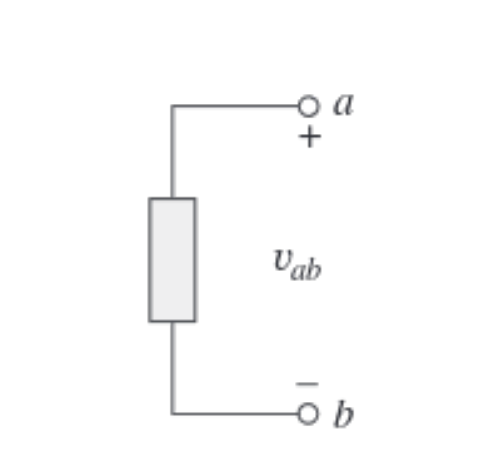
\includegraphics[height=0.15\textwidth]{./fig/fig2.png}
	\caption{Polaridade da tensão \( v_{ab} \).}
	\label{fig:fig2}
\end{figure}

Segue-se logicamente então que:

\[
	v_{ab} = -v_{ba}
\]

Uma tensão CC é comumente produzida por uma bateria e é representada por V e uma
tensão CA é produzida por um gerador elétrico sendo representada por v.
